%! TeX root: ../thesis_a4.tex

% Clickable link from each RO mention to the consolidated table.
% (Ideally move this \newcommand to the preamble/main.tex.)


\chapter{Introduction}
\label{ch01_intro}

%Audio processing is a subfield of signal processing with application areas that can range from speech processing to music synthesis. Traditionally, audio processing research has consisted of finding analytical solutions to signal problems. However, in the last decade with the advent of \acrshortpl{DNN}, the field has shifted from an analytical to a data-driven approach, bringing unprecedented performance in numerous audio-related tasks such as retrieving specific elements from an audio mixture (source separation) and removing noise (denoising) or reverberation (dereverberation) to improve quality and/or intelligibility of speech signals.

% =====================================================================
% Chapter 1 — Introduction
% Draft following the agreed outline (1.1 Context, 1.2 Motivation,
% 1.3 Industrial PhD, 1.4 Outline & Research objectives).
% Citation keys are placeholders: align them with your .bib.
% Items marked % CITE need a source you must supply/verify.
% =====================================================================


Audio processing is the subfield of signal processing concerned with the
analysis, modification, and generation of sound signals. Historically, its
applications have grown around several research communities, some of which this thesis touches upon: the \emph{speech} field, devoted to understanding, transcribing and enhancing spoken language; the \emph{machine listening} field, which studies how to extract information about the acoustic environment; the \emph{computational audiology} field, which studies how to compensate for hearing loss and improve listening in adverse conditions; the \emph{music} field, where the retrieval and manipulation of musical content is studied under the umbrella of \acrfull{MIR}; and the \emph{acoustic signal processing} field, which encompasses the full range of audio tasks, among others. The work in this thesis sits at the intersection of these communities, several of whose most representative tasks are listed in Table~\ref{tab:tasks}.

Until the last decade, these communities have relied on analytical, hand-engineered solutions grounded in acoustics, psychoacoustics and
statistical signal processing. However, the advent of deep learning \citep{lecun2015deep} has reshaped all of them, shifting the dominant paradigm from
explicit modelling to data-driven learning, bringing unprecedented performance, especially in tasks where analytical approaches are limited. This has led to significant advances in tasks such as retrieving specific elements from an audio mixture (source separation) and removing noise (denoising) or reverberation (dereverberation) to improve quality and/or intelligibility of signals, and has also given rise to new tasks and interfaces previously unfeasible, such as text-to-audio. 

These tasks (listed in Table~\ref{tab:tasks}) can be grouped into three paradigms: those that \emph{categorise} audio content---such as tagging or key detection; those that \emph{infer} a structured output from the signal---such as source separation or \acrshort{SE}; and those that \emph{generate} new audio---such as speech synthesis or text-to-music. These paradigms correspond, respectively, to the machine learning problems of \emph{classification}, \emph{regression}, and more recently to the \emph{sampling} of generative models. Although the contributions of this thesis may prove useful across all three paradigms, it particularly focuses on a subset of the regression-oriented family of tasks, which we refer to as \emph{audio processing} tasks, in the sense that both the model's inputs and outputs are audio signals and to differentiate them from \emph{audio analysis} and \emph{audio generation} models. 

In the present work, we focus on three of these representative tasks, the choice of which is also motivated by the industrial partners involved in the thesis, and each one from a distinct audio research field: \textbf{\textit{(i)}~\acrfull{SE}} from the speech field, \textbf{\textit{(ii)}~\acrfull{MSS}} from the \acrfull{MIR} field, and \textbf{\textit{(iii)}~\acrfullpl{HA}} processing from the computational audiology field. 

\begin{table}[t]
\centering
\begin{tabular}{p{0.18\textwidth}|p{0.28\textwidth}|p{0.44\textwidth}}
\makecell[cc]{\textbf{Field}} & \makecell[cc]{\textbf{Venues}} & \makecell[cc]{\textbf{Representative tasks}} \\
\hline
\makecell[l]{Acoustics} & \makecell[l]{ICASSP  \\WASPAA\\EUSIPCO} & \makecell[l]{DoA estimation \\ Beamforming \\ Echo cancellation \\ \acrshort{RIR} estimation} \\
\hline
\makecell[l]{Speech} & \makecell[l]{Interspeech \\ ASRU\\ICASSP\\WASPAA } & \makecell[l]{\acrshort{ASR} \\ Speaker verification \\ \acrshort{SE} \\ Text-to-Speech \\ Voice conversion} \\
\hline
\makecell[l]{Machine \\listening} & \makecell[l]{DCASE \\ ICASSP \\ WASPAA} & \makecell[l]{Acoustic scene classification \\ Sound event detection \\ Audio moment retrieval \\ Sound localisation} \\
\hline
% Fixed: Removed the trailing \\ after audiology
\makecell[l]{Computational \\audiology} & \makecell[l]{VCCA \\ AES \\ EMBC \\ ICASSP\\WASPAA} & \makecell[l]{\acrshortpl{HA} processing \\ Cochlear implant processing \\Noise reduction \\ Speech intelligibility prediction \\ Hearing loss simulation} \\
\hline
\makecell[l]{\acrshort{MIR}} & \makecell[l]{ISMIR \\ SMC \\ICASSP\\WASPAA} & \makecell[l]{Beat tracking \\ Chord recognition \\ Source separation \\ Transcription \\ Text-to-song} \\
\end{tabular}
\caption{Some representative audio processing tasks for each research community and the main venues where they are traditionally presented. This selection is merely illustrative and intended to contextualise the thesis within the broader audio processing landscape; it is by no means exhaustive, and the tasks are not mutually exclusive --- for example, source separation is relevant to both the acoustics and music fields. A more comprehensive taxonomy can be found in \citep{huang2025dynamic}.}
\label{tab:tasks}
\end{table}


\section{Context}
\label{sec:context}

To situate the contributions of this thesis within the context of audio processing, we first trace the transition from analytical to data-driven methods, which has unfolded along two axes. The first concerns the signal representations. Models
that used to operate on hand-crafted descriptors built from expert
domain knowledge have progressively given way to architectures that learn their own representations directly from time--frequency transforms or even from the raw waveform \citep{pons2019}. These learned representations have themselves grown more abstract: continuous, high-dimensional feature maps have transitioned to discrete latent codes, learned end-to-end and quantised into a finite vocabulary. Neural audio codecs epitomise this shift, compressing the waveform into a handful of discrete tokens that preserve perceptual fidelity
\citep{zeghidour2021soundstream,defossez2022high} while exposing a tokenised
substrate over which language-model architectures can operate directly
\citep{borsos2023audiolm}. Continuous latent spaces have remained equally
productive, most notably the encoder-decoder structure of the Variational Auto Encoder (VAE) that underpins latent-diffusion
generative models such as \citet{evans2025stable}, where a
compressed continuous latent serves as the domain over which the generative
process is defined. However, these models work at a latent rate in the order of $\sim$10 to 20~Hz, so the compactness of the representations intrinsically makes them hard to deploy in real time due to their latency constraints (with some exceptions such as \citealp{gdmlyria2025live,novack2025fast}).

The second axis concerns another recent inflection, visible across machine learning as a whole, which is the move from purely supervised training towards large-scale self- and semi-supervised \emph{pre-training}. Instead of training a model from scratch for a single task, the encoder-decoder model is first trained on vast amounts of unlabelled or weakly labelled data to learn general-purpose representations by contrastive or masking approaches, and only then is adapted to specific downstream tasks, usually by adding task-specific layers. The resulting models, often termed \emph{foundation models}, have delivered remarkable performance in Natural Language Processing (NLP) \citep{devlin2019bert, touvron2023llama} and are increasingly replicated in the audio and speech domains \citep{baevski2020wav2vec2, mohamed2022ssl}, but they are usually bound to large parameter counts and inference budgets that also make them difficult to deploy in real time and on consumer-grade hardware, and that are particularly problematic for wearable applications such as \acrfullpl{HA}.

Likewise, the trajectory from analytical methods to learned, increasingly end-to-end models and with weaker supervision has been observed across the three fields we address. 

\textbf{\textit{(i)}~In the \emph{speech} field}, classical \acrfull{ASR} used Mel-Frequency Cepstral Coefficients \citep{davis1980mfcc} feeding statistical
acoustic models \citep{rabiner1989tutorial}, an approach later overtaken by \acrshort{DNN} acoustic modelling
\citep{hinton2012} and, more recently, by large end-to-end models such as
Whisper, trained on hundreds of thousands of hours of weakly supervised audio
\citep{radford2022whisper}. 

\textbf{\textit{(ii)}~In the \emph{music} field}, source separation was long
dominated by analytical decompositions such as non-negative matrix
factorisation \citep{virtanen2007nmf}, before being superseded by \acrshort{DNN}-based
systems exemplified by open, reproducible baselines such as Open-Unmix \citep{stoter2019openunmix}. 

\textbf{\textit{(iii)}~In the \emph{computational audiology} field}, traditional methods of \acrshortpl{HA} improve the signal-to-noise ratio through directional microphones and adaptive beamforming
\citep{ricketts1999, gode2022}, techniques rooted in array signal processing
and typically validated under controlled laboratory conditions. More recently,
Deep Neural Networks (\acrshortpl{DNN}) have been proposed as enhancement back-ends for
\acrshortpl{HA} for binaural separation \citep{han2020}, or as evaluation metrics \citep{chiang2024multi}, with recent interest in distillation to smaller models that are compatible with wearable constraints
\citep{wang2023neural, andersen2021}.



Both axes and examples point in the same direction: towards models that are more powerful and capable of tasks unthinkable a decade ago, but at a steep computational cost.
The representations are richer and the pre-trained backbones larger, yet this
capability is increasingly bought with parameter counts and inference budgets
that place these models out of reach for local or consumer-grade hardware, and
that make real-time deployment difficult. This thesis explores an alternative
direction. Rather than chasing capability through ever-larger models trained on
ever-more data, can we displace part of the complexity onto the selection and
construction of the training data, while keeping model size fixed? Put differently: \textbf{can \emph{better} data --- more representative of the conditions a
model will actually face --- improve performance without resorting to more data and larger models?}





\section{Motivation: the importance of ecological validity}
\label{sec:motivation}
In this section, we lay out two examples that have motivated the data-centric direction this thesis pursues. We have mentioned that \acrshort{DNN}-based audio processing performs extremely well on many tasks. This performance is traditionally measured on benchmark datasets the community
has standardised around, and progress on these benchmarks is pursued so
relentlessly that successive systems have \emph{saturated} them. By saturation we mean that performance gains have largely plateaued, so that further improvements demand disproportionately more compute and parameters for diminishing returns. We illustrate this for the two-speaker speech separation task and the progress of the \acrfull{SOTA} across the last decade, which we depict in Figure~\ref{fig:wsj0_2mix_sota}.

\begin{figure}[htbp]
    \centering
    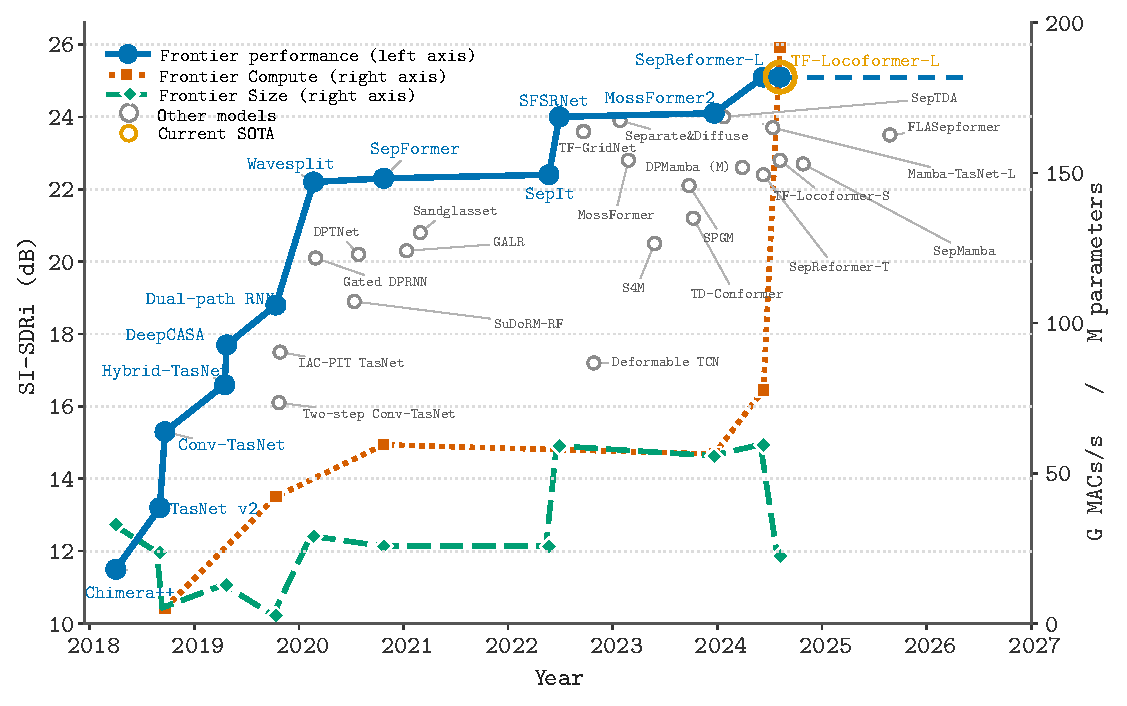
\includegraphics[width=\textwidth,trim={.25cm .25cm .25cm .25cm},clip]{ch01_introduction/figures/wsj0_2mix_sota_v6.pdf}
      \caption{Progress on clean two-speaker speech separation over the last decade,
      evaluated on the WSJ0-2mix test set. Each marker is a published model: grey
      markers are individual systems, and blue markers trace the
      \emph{frontier} of performance --- the \acrshort{SOTA} \acrshort{SI-SDR}i at each
      point in time (left y-axis), with the current \acrshort{SOTA} highlighted. The
      orange and green lines (right y-axis) report the computational cost and model
      size of the frontier models for which such data was available, expressed in
      \acrshort{GMACs}/s and millions of parameters, respectively. While performance
      has plateaued around 22~dB, compute and size have continued to grow, illustrating
      the saturation discussed in the text. Computational figures are taken from
      \citep{wang2025flasepformer}.}
    \label{fig:wsj0_2mix_sota}
\end{figure}
\vspace{0.8cm}
Speech separation performance is commonly measured by the \acrfull{SI-SDR} proposed by \citet{le2019sdr}, which quantifies the similarity between the separation estimate and a reference ground truth source signal, usually reported as improvement upon the mixture (denoted with the \textit{i} in \acrshort{SI-SDR}i). Traditionally, the speech community has used the WSJ0-2mix dataset \citep{hershey2016deepclustering} to assess progress on clean speech separation and to compare with previous existing literature. \acrshort{SOTA} performance over time shows that progress is increasingly hard, and although the saturation seemed more pronounced at the beginning of this thesis (around 2022, where performance progress had largely stalled), the performance leaps that have been made in \citet{rixen2022sfsrnet} and \citet{shin2024separate} grow smaller every time. Note also how the computational cost, here measured in terms of the number of matrix multiplications per second, is also increasing. As a rule of thumb, an \acrshort{SI-SDR}i >20dB is often taken for near-perfect separation, which was already achieved in 2022.  

However, this apparent progress can be misleading: when the same models are
evaluated across datasets (cross-dataset evaluation), performance often degrades
sharply, revealing that they have, to a large extent, overfit to the
idiosyncrasies of a particular dataset rather than generalised to unseen
conditions --- learning to exploit dataset-specific artefacts rather than the
underlying task, a failure mode memorably diagnosed in the music domain by
\citet{sturm2017horse}. Continuing with the two-speaker clean speech
separation example, \citet{kadiouglu2020empirical} proposed cross-dataset
evaluation and showed that a Conv-TasNet trained on WSJ0-2mix degrades sharply on
LibriTTS and vice-versa, as we depict in Figure~\ref{fig:convtasnet_xdataset}.
A similar pattern holds for tasks other than separation: \acrshort{SE} models
trained on one dataset degrade on others, in their case due to channel and
recording-condition mismatch \citep{pandey2020crosscorpus}.

\begin{figure}[htbp]
    \centering
    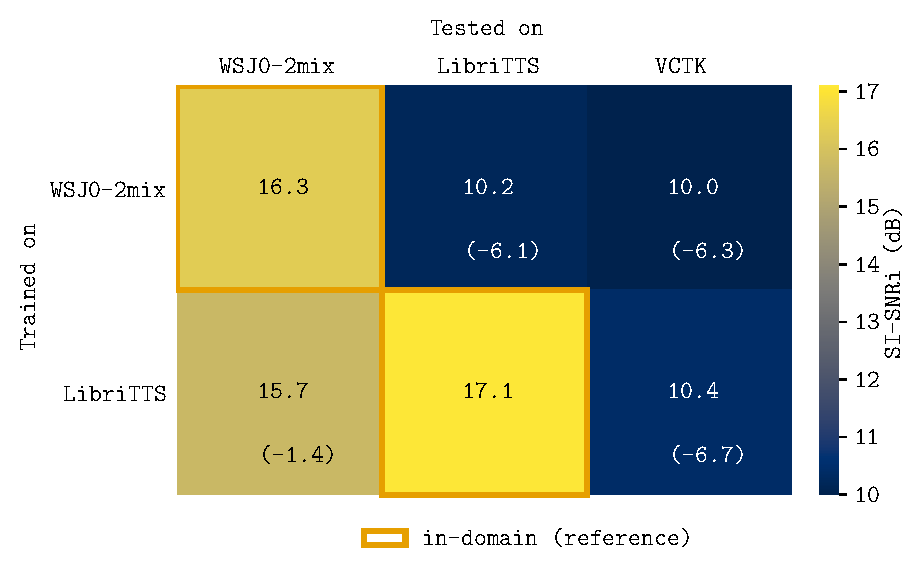
\includegraphics[width=0.8\textwidth]{ch01_introduction/figures/xdataset_matrix.pdf}
      \caption{Cross-dataset generalisation of Conv-TasNet on two-speaker speech
      separation, reported in SI-SNRi (dB) in the original study. Each row corresponds to the
      training dataset and each column to the test set; diagonal cells, outlined in
      orange, are in-domain (matched train/test) references. Off-diagonal cells report
      out-of-domain performance, with the drop relative to the corresponding in-domain
      reference shown in parentheses. Models trained on one corpus lose roughly 6~dB
      when evaluated on a different one (e.g.\ $-6.1$ and $-6.3$~dB for the WSJ0-2mix
      model on LibriTTS and VCTK), illustrating that high in-domain scores do not
      transfer across datasets. Values taken from \citet{kadiouglu2020empirical}.}
    \label{fig:convtasnet_xdataset}
\end{figure}

We frame this gap through the notion of \textbf{\emph{ecological validity}}. The
term was originally introduced in psychology by Egon Brunswik \citep{brunswik1955}
with a narrow, technical meaning: within his lens model of perception, it
denoted the statistical reliability of a perceptual cue. In its contemporary and considerably broader usage, however, the term
has come to mean something Brunswik did not intend: the extent to which findings
obtained under controlled laboratory conditions generalise to real-life
settings \citep{leglaive2023chime}. We adopt this modern sense throughout this thesis.

Transposed to supervised audio processing, ecological validity concerns the
degree to which the training and evaluation data reproduce
the acoustic conditions of the intended deployment scenario: realistic noise
and reverberation, source and receiver directivity, room and venue acoustics,
transducer responses, and so on. From this perspective, saturating a benchmark
is a perfectly legitimate measure of progress, but it must be complemented by
evaluations that are themselves ecologically valid, so that gains
translate into the real world.

A complementary, more quantitative view of the same gap comes from the machine
learning literature, where it is studied under the notion of \emph{domain
mismatch} (or \emph{distribution shift}). Supervised models are trained under the
implicit assumption that training and real data are drawn from the same underlying distribution; when this assumption is violated performance degrades, often severely \citep{quinonero2008dataset}. The same concern was raised canonically in computer vision by \citet{torralba2011unbiased}, who showed that models trained on one dataset generalise poorly to others because they absorb each dataset's particular biases. In audio processing, this mismatch is rarely a single
factor but the compound effect of many: the recording channel and microphone
response, room acoustics and reverberation, the noise types and signal-to-noise
ratios present, speaker or instrument characteristics, and the way mixtures are
constructed in synthetic benchmarks. The cross-dataset degradation reported above
(Figure~\ref{fig:convtasnet_xdataset} and the channel-mismatch effects of
\citealp{pandey2020crosscorpus}) are concrete examples of this shift. Reducing domain mismatch and improving ecological validity are thus two
framings of a single objective, and the one this thesis pursues: aligning the
data a model is trained and evaluated on with the conditions of its intended use.

This intuition can be made precise. Let $\mathcal{X}$ denote the space of input
signals and $\mathcal{Y}$ the space of targets (separated sources/instruments, enhanced speech,
etc.), and let a model $f_\theta : \mathcal{X} \rightarrow \mathcal{Y}$ be trained
to minimise the expected loss $\mathcal{L}$ over a \emph{source} domain
$p_S(x, y)$:
\begin{equation}
    \theta^\star = \arg\min_\theta \;
    \mathbb{E}_{(x,y)\sim p_S}\!\left[\mathcal{L}\!\left(f_\theta(x), y\right)\right].
    \label{eq:erm}
\end{equation}
At deployment, however, the model is evaluated on a \emph{target} distribution
$p_T(x, y)$, and the quantity we actually care about is the target risk
$\mathbb{E}_{(x,y)\sim p_T}[\mathcal{L}(f_{\theta^\star}(x), y)]$. Empirical risk
minimisation offers guarantees only when $p_S = p_T$; \emph{domain mismatch} is
precisely the condition
\begin{equation}
    p_S(x, y) \neq p_T(x, y),
    \label{eq:mismatch}
\end{equation}
under which a model optimal on the source domain need not be optimal---or even
adequate---on the target domain. 

We can factorise the joint
distribution as $p(x, y) = p(x)\,p(y \mid x)$. In the audio processing tasks we
consider, the conditional input--output relationship is largely physical and
stable across domains (e.g.\ the mapping from a noisy mixture to its clean
elements is governed by the same acoustics everywhere), so $p_S(y \mid x) \approx
p_T(y \mid x)$, and the dominant discrepancy lies in the marginal over inputs,
$p_S(x) \neq p_T(x)$. Each benchmark fixes a particular $p(x)$---a specific
distribution of channels, rooms, noises and speakers---and the cross-dataset
degradation reported above is the gap between performance under $p_S(x)$ and under
a different $p_T(x)$. The contributions of this thesis can be read
as efforts to bring the training input distribution $p_S(x)$ closer to the
deployment distribution $p_T(x)$ through the selection and construction of
training data. Several broad strategies exist to mitigate this mismatch. 

A first family acts on the
model: \emph{domain adaptation} techniques adjust a trained model towards the target domain, often using small amounts
of unlabelled target data \citep{hsu2017unsupervised}. A second, radically different response to domain mismatch is simply to enlarge the
training distribution until it subsumes the deployment one. Rather than adapting
to a specific target, one trains a single large model on a corpus so vast and
heterogeneous that few conditions remain genuinely out-of-distribution; the
target $p_T(x)$ then falls within the support of an enormous $p_S(x)$. This is the
logic behind large-scale weak supervision in speech: \citet{radford2022whisper},
for instance, train on hundreds of thousands of hours of diverse web audio and
obtain strong \emph{zero-shot} robustness across datasets, attributing the gain to
data diversity rather than to any adaptation mechanism. From the perspective of
the previous paragraphs, this is a brute-force way of minimising the gap between
$p_S(x)$ and $p_T(x)$---not by carefully shaping $p_S(x)$, but by making it large
enough to cover everything.

This strategy is remarkably effective, but it is precisely the one that the
constraints of this thesis rule out; the parameter counts and inference budgets
inherent to web-scale training are incompatible with the real-time, on-device
deployment targets that motivate our work. When scaling the model and the data
is not an option, the quality and representativeness of a fixed-size training
set become the primary lever --- which returns us to ecological validity. This
constraint also shapes the very \emph{choice} of problems studied in this
thesis. Every experiment reported here was run on a single \acrfull{GPU}, so we
have deliberately favoured tasks where progress comes from improving the
\emph{data} rather than from scaling the model: the design of ecologically valid
evaluations and the construction of better training datasets, where a small
group can still make a measurable difference.

\section{Industrial PhD}
\label{sec:industrial}

The choice of the specific tasks in which we investigate towards improving ecological validity has been motivated by the partners involved in this PhD. This dissertation has been carried out as an \emph{industrial PhD}, a doctoral modality designed to bridge academia and industry by embedding the doctoral candidate within a company or organisation while maintaining a formal partnership with a university or research centre. Unlike a traditional academic PhD — which primarily advances knowledge within a scientific discipline — an industrial PhD aligns research objectives with the strategic needs of the industrial partner, targeting outcomes such as technological innovation, process improvement, or competitive advantage. The candidate operates across both environments simultaneously, contributing to the partner's goals while producing original research that culminates in a doctoral thesis.

From the academic side, the Music Technology Group (MTG) at the Universitat Pompeu Fabra (UPF) in Barcelona is one of the leading research groups in sound and music computing worldwide. Founded in 1994 within UPF's Department of Information and Communication Technologies, and now part of the Department of Engineering, the MTG conducts research spanning signal processing, machine learning, music perception, computational musicology, and human-computer interaction, with applications ranging from music creation and performance to education and cultural heritage. A defining characteristic of the group is its commitment to open science: flagship initiatives such as Freesound, a collaborative repository of Creative Commons audio samples, and Essentia, an open-source library for audio analysis and music description, have become widely adopted tools in both the research community and industry. The MTG has grown into an interdisciplinary team that combines scientific rigour with artistic and societal relevance, and maintains active collaborations with musicians, educators, and industry partners.

From the industrial side, Eurecat is a foundation whose mission is to promote research, technological development, and knowledge transfer in order to improve the competitiveness of companies and the well-being of society. It was created in 2015 through the consolidation of several industrial research units from across Catalonia. The audio research group at Eurecat traces its origins to Barcelona Media, a foundation for innovation and interdisciplinary research that operated from 2002 and developed solutions across a broad range of technological domains, including image, audio, and social media analysis. Among its most notable achievements, the Barcelona Media audio team developed the immersive 3D audio technology behind Imm Sound, a cinema sound solution acquired by Dolby Laboratories in 2012. The researchers who remained at Barcelona Media after that acquisition formed the core of what would become Eurecat's audio group when the centre was established in 2015.

Three Eurecat projects underpin the work presented in this thesis.

\begin{itemize}{
    \item \textbf{Eurecat-Microson} collaboration project, focusing on the development of a new benchmark for evaluating \acrshortpl{HA} and speech denoising algorithms in realistic conditions.
    
    \item \textbf{GuestXR} (Horizon 2020) project, aimed at creating an immersive online social space through extended reality, centred on a machine learning agent called ``The Guest'' designed to facilitate interaction between participants, mitigate conflicts and cyberbullying. Because supporting participants with and without hearing difficulties requires intelligible speech, our contribution addresses \acrshort{SE}.

    \item \textbf{Traça IAGen}, an internal Eurecat initiative funded by the Catalan Government with the goal of driving the adoption of generative AI across the centre's different research units.
}
\end{itemize}



\section{Research objectives and thesis outline}
\label{sec:outline}

In light of the above, this thesis investigates whether improving the
ecological validity of (often synthetic) training and evaluation data is an
effective lever for closing the generalisation gap, across three audio
processing tasks --- one per partner and field. The remainder of the manuscript tackles the following Research Objectives (RO) summarised in
Table~\ref{tab:research_objectives} and expanded, chapter by chapter, in the
outline below.

\begin{table}[hb]
\centering
\footnotesize
\renewcommand{\arraystretch}{1.3}
\begin{tabular}{@{}p{0.055\textwidth} p{0.16\textwidth} p{0.68\textwidth}@{}}
\toprule
\textbf{RO} & \textbf{Field (Chapter)} & \textbf{Research objective} \\
\midrule
RO1 & \acrshortpl{HA} \newline (Ch.~\ref{ch03_hearing})
    & An ecologically valid \emph{evaluation} of \acrshort{HA} \acrshort{SE} in complex scenes. \\
RO2 & \acrshortpl{HA} \newline (Ch.~\ref{ch03_hearing})
    & Do \acrshortpl{DNN} outperform and generalise better than traditional \acrshort{HA} algorithms? \\
\midrule
RO3 & Monaural \acrshort{SE} \newline (Ch.~\ref{ch04_mbrirs})
    & Do \acrshortpl{RIR} generated with frequency-dependent absorption coefficients and source/receiver directivity improve the generalisation of monaural \acrshort{SE} models to real data? \\
RO4 & Monaural \acrshort{SE} \newline (Ch.~\ref{ch04_mbrirs})
    & Do fewer but geometrically more realistic mesh-based \acrshortpl{RIR} improve \acrshort{SE} performance over abundant shoebox ones? \\
\midrule
RO5 & \acrshort{MSS} \newline (Ch.~\ref{ch05_mss})
    & Bring \acrshort{MSS} to the concert setting by generating synthetic audiences that sing along to the studio vocals through a generative singing-voice conversion model. \\
RO6 & \acrshort{MSS} \newline (Ch.~\ref{ch05_mss})
    & Curate additional audience-like noise from freely available internet audio archives. \\
RO7 & \acrshort{MSS} \newline (Ch.~\ref{ch05_mss})
    & Determine whether impulse responses measured in real, modern concert venues improve upon existing non-concert \acrshortpl{RIR}. \\
\bottomrule
\end{tabular}
\caption{The seven Research Objectives (RO) addressed in this thesis.}
\label{tab:research_objectives}
\end{table}

\begin{itemize}
    \item \textbf{Chapter~\ref{ch02_sota}} introduces the scientific background used broadly throughout the thesis: deep-learning for audio, spatial-audio techniques and virtual-acoustics on which the contributions build, together with a summary of their corresponding publicly available datasets.
    
    \item \textbf{Chapter~\ref{ch03_hearing}} addresses the \acrshortpl{HA} field and is the result of the collaboration with Microson and within the GuestXR project: the development of an ecologically-valid \emph{evaluation} for \acrshortpl{HA} (\RO{1}), and whether \acrshortpl{DNN} are a promising route to generalise better than traditional \acrshortpl{HA} algorithms (\RO{2}). Beyond their technical interest, both objectives foster accessibility, and thus inclusivity, for people with hearing loss.

    \item \textbf{Chapter~\ref{ch04_mbrirs}} carries the idea to more general models, again part of the GuestXR project. It investigates whether \acrfull{RIR}s generated with frequency-dependent absorption coefficients and source or receiver directivity improve the generalisation of monaural \acrfull{SE} models to real data (\RO{3}), and, in pursuit of the same ecological validity, whether using fewer but more realistic mesh-based \acrshort{RIR}s improves performance (\RO{4}). While large, realistic \acrshort{RIR} datasets already exist privately within industry --- where major labs maintain their own simulation tools --- replicating them for open science and releasing them freely to every research lab carries value in itself.

    \item \textbf{Chapter~\ref{ch05_mss}} brings the same idea to \acrfull{MSS}, in line with the research interests of the MTG (UPF). We identify that \acrfull{SOTA} models designed for studio music do not work well on recordings captured by attendees (mobile-phone recordings from the audience). This raises several questions: can we generate synthetic data that transforms studio datasets into live datasets? Can a generative singing-voice conversion model produce synthetic audiences that sing along to the vocals of the studio songs (\RO{5})? Can we curate additional audience-like noise from internet audio archives (\RO{6})? And what about acoustics --- does adding impulse responses specifically measured in real, modern music venues improve upon using existing non-concert \acrshort{RIR}s (\RO{7})?

    \item \textbf{Chapter~\ref{ch98_conclusions}} closes the dissertation with some additional discussion, general conclusions and perspectives for future work.

    \item We provide a list of publications (Appendix \ref{sec:pubs}) and research materials (Appendix \ref{app:materials}).

\end{itemize}

Having grounded the concepts of \acrshort{DNN}-based \emph{audio processing} and \emph{ecological
validity}, the title of this thesis can now be read in full: our aim is to
improve the ecological validity of datasets as a lightweight route to
better-generalising, deployable audio processing models---one per project of
this Industrial PhD.